I dette kapitel unders�ges hvordan funktioner til videoapplikationen ville se ud, hvis ikke skulle hente deres data fra et XML dokument, men i stedet hente dataene direkte fra tabeller i en relationel database. Resultatet af et funktionskald skal dog stadig v�re i form af et resultats�t beskrevet med XML.

Databasen som vil blive brugt i dette projekt er en PostgreSQL database og der arbejdes udelukkende med data fra XML dokumentet programseries.xml.

\section{Design af tabeller}

F�rste opgave er at designe nogle tabeller, som kan underst�tte indholdet i XML dokumentet. Den f�rste tabel, der skal bruges er en tabel til at holde p� selve XML dokumentet i sin komplette tilstand. Til det form�l er tabellen �downloadedXML� oprettet. Denne tabel indeholder to kolonner, en til navnet p� XML dokumentet (docmentTitle) og en til selve indholdet af dokumentet (documentContent) som er af typen XML.

Fra unders�gelsen af programseries.xml, tilbage i kapitel 2.2, er det allerede kendt at der findes en 0 til mange relation imellem en programserie og programserien's label's, alts� kategorier. I figur \ref{postgresql:ER-diagram} ses et ER-diagram, som viser denne relation.  Derfor er der oprettet en tabel udelukkende til labels og en tabel udelukkende til indholdet af en programserier. Til at beskrive relationen, at en programserie har 0 til mange label�s og at label�s har 0 til mange programserier, s� er der oprettet en tabel, som hedder slugLabel, der har en reference til label-tabellen og en reference til programserie-tabellen. Dermed er denne relation beskrevet i databasen og tabellerne er nu klar til at f� indl�st data i sig.

\begin{figure}[ht]
  \centering
   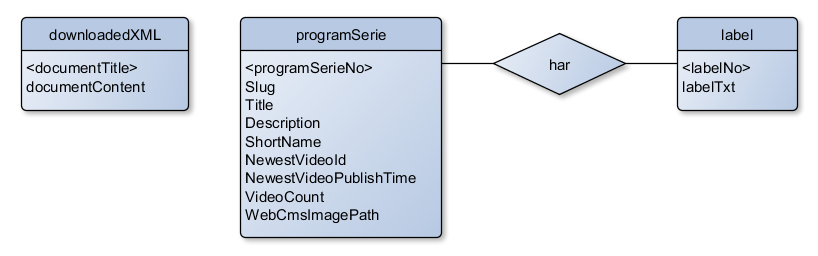
\includegraphics[width=1.1\textwidth]{pic/ER_programserie.png}
   \caption{ER-diagram over tabel-design.}
   \label{postgresql:ER-diagram}
\end{figure}

\section{Oprettelse af label�s}

N�r XML dokumentet er indl�st i tabellen downloadedXML, s� skal der som det f�rste oprettes label's til alle de kategorier, som findes i dokumentet programseries.xml. Til dette form�l er funktionen getAndInsertAllLabels(), som ses i figur \ref{code:getAndInsertAllLabels} skabt. Denne funktion benytter et XPath-udtryk til at finde alle tekster til label's og for hver tekst den finder, s� unders�ges det om der allerede er oprettet en label med denne tekst, hvis ikke, s� inds�ttes denne nye label i tabellen. 

\begin{figure}[h]
\centering
\begin{lstlisting}[style=SQL]
  labels := (SELECT xpath('//ProgramSerie/Labels/string/text()', 
             downloadedXML.documentContent) FROM downloadedXML);
  FOR i IN array_lower(labels, 1) .. array_upper(labels, 1)
  LOOP
    SELECT labelNo INTO v_found FROM label WHERE label.labelTxt = labels[i];
    IF v_found IS NULL THEN
      INSERT INTO label(labelTxt) VALUES(labels[i]);
    END IF;
  END LOOP;
\end{lstlisting}
\caption{Udsnit af funktionen getAndInsertAllLabels()}
\label{code:getAndInsertAllLabels}
\end{figure}

\section{Oprettelse af programserier samt label relationer}

For at identificere alle programserier, s� er funktionen getAndInsertAllSlugs() implementeret. Denne funktion finder med et XPath-udtryk alle programseriers \ele{slug} tag�s indhold og sender det videre til funktionen getAndInsertSlugsDetail(), som har til opgave et hente detaljerne ud og oprette relationer imellem programserierne og deres eventuelle label�s. Denne funktion ses i figur \ref{code:getAndInsertSlugsDetail}.

\begin{figure}[h]
\centering
\begin{lstlisting}[style=SQL]
CREATE OR REPLACE FUNCTION getAndInsertSlugsDetail(p_slug VARCHAR) RETURNS VARCHAR AS $$
<< outerblock >>
DECLARE
  v_title                   text;
  v_description             text;
  v_shortName               text;
  v_newestVideoId           integer;
  v_newestVideoPublishTime  timestamp without time zone;
  v_videoCount              integer;
  v_webCmsImagePath         text;
  v_tag_value               text[];
  v_labels                  text[];
  v_programSerieNo          integer;
  v_labelNo                 integer;
BEGIN
  v_tag_value := (SELECT xpath('//ProgramSerie[Slug='''|| 
                  p_slug ||''']/Title/text()', 
                  downloadedXML.documentContent) FROM downloadedXML);
  v_title := v_tag_value[1];
  v_tag_value := (SELECT xpath('//ProgramSerie[Slug='''|| 
                  p_slug ||''']/Description/text()', 
                  downloadedXML.documentContent) FROM downloadedXML);
  v_description := v_tag_value[1];
  /**********************************************************/
  /* ...... samme metode for resten af variabelerne ....... */
  /**********************************************************/
  v_tag_value := (SELECT xpath('//ProgramSerie[Slug='''|| p_slug 
                  ||''']/WebCmsImagePath/text()', 
				  downloadedXML.documentContent) FROM downloadedXML);
  v_webCmsImagePath := v_tag_value[1];    
  INSERT INTO programSerie (Slug, Title, Description, ShortName, NewestVideoId, 
                            NewestVideoPublishTime, VideoCount, WebCmsImagePath)
  VALUES (p_slug, v_title, v_description, v_shortName, v_newestVideoId, 
          v_newestVideoPublishTime, v_videoCount, v_webCmsImagePath)
  RETURNING programSerie.programSerieNo INTO v_programSerieNo;

  v_labels := (SELECT xpath('//ProgramSerie[Slug='''|| p_slug 
               ||''']/Labels/string/text()', 
               downloadedXML.documentContent) FROM downloadedXML);
  IF array_lower(v_labels, 1) IS NOT NULL THEN
    FOR i IN array_lower(v_labels, 1) .. array_upper(v_labels, 1)
    LOOP
      SELECT labelNo INTO v_labelNo FROM label WHERE label.labelTxt = v_labels[i];
      IF v_labelNo IS NOT NULL THEN
        INSERT INTO slugLabel (programSerieNo, labelNo) 
		VALUES(v_programSerieNo, v_labelNo);
      END IF;
    END LOOP;
  END IF;
  RETURN v_title;
END;
$$ LANGUAGE plpgsql;
\end{lstlisting}
\caption{Funktionen getAndInsertSlugsDetail()}
\label{code:getAndInsertSlugsDetail}
\end{figure}

\section{Funktionen til at finde programserier med specifik label}

Til videoapplikationen skal der som tidligere n�vnt bruges en funktion, som kan give et resultats�t af programserier inden for en given kategori, alts� med en specifik label. Til det form�l er funktionen programseriesOfLabel() implementeret. Den tager kategori navnet som argument og er vist i figur \ref{code:programseriesOfLabel}. Den efterspurgte information er fordelt p� tre tabeller i PostgreSQL databasen som er: label, sluglabel og programserie.  
I denne funktion blev der anvendt et cross join imellem de tre tabeller med efterf�lgende WHERE betingelse for at finde alle programserier igennem deres programserieno, som er registreret i tabellen sluglabel p� den efterspurgte label. Resultatet skal returneres formateret som XML og skal kun vise nogle af kolonnerne fra programserie-tabellen. De indbyggede PostgreSQL funktioner XMLRoot(), XMLAgg() og XMLElement() blev brugt og genererer et velformet XML dokument med rodelement \ele{programseries}, som indeholder de fundende elementer af \ele{programserie}. XML dokumentet mangler en DTD eller et XML skema og den tilh�rende prolog for at blive et valid XML dokument.

\begin{figure}[h!]
\centering
\begin{lstlisting}[style=SQL]

CREATE FUNCTION programseriesOfLabel(labelName character(50) ) returns SETOF xml
AS $$
DECLARE

BEGIN
  
RETURN QUERY 
  SELECT XMLRoot(
    (SELECT XMLElement( name "programseries",
    XMLAgg( XMLElement( name "programserie",
        XMLElement( name "slug", ps.slug),
        XMLElement( name "titel", ps.title),
        XMLElement( name "description", ps.description),
        XMLElement( name "newestvideoid", ps.newestvideoid),
        XMLElement( name "newestvideopublishtime", ps.newestvideopublishtime)
        ) 
      )
    )
    
  FROM   programserie ps, sluglabel sla, label la
  WHERE  la.labeltxt = labelName
  AND    sla.labelno = la.labelno
  AND    sla.programserieno = ps.programserieno
  ), VERSION '1.0', STANDALONE yes
  );
  
END;
$$
LANGUAGE plpgsql;

\end{lstlisting}
\caption{Funktionen til at finde programserier registreret under en specifik kategori.}
\label{code:programseriesOfLabel}
\end{figure}



\section{Funktionen til at finde programserier i et tidsinterval}

En yderlige funktion figur \ref{code:programseriesByPublishInterval} blev implementeret, som g�r det muligt at s�ge efter programserier, som blevet offentliggjort i et specifikt tidsinterval. Igen skal der returneres nogle kolonner af de fundet programserier, men denne gang sorteret med de nyeste programserier f�rst. En ORDER BY kommando sorterer de fundet programserier med hensyn til kolonnen newestvideopublishtime inden de bliver udgivet pakket ind i XML. Aggregationsfunktionen XMLAgg() og ORDER BY i SQL-foresp�rgselen resulterer i en yderlige SELECT statement og dermed dybere nested SQL funktion. Med hj�lp af funktionen XMLRoot() returneres et velformet XML dokument. 


\begin{figure}[h!]
\centering
\begin{lstlisting}[style=SQL]
CREATE FUNCTION programseriesByPublishInterval(startTime timestamp, stopTime timestamp ) returns SETOF xml
AS $$
DECLARE

BEGIN
  RETURN QUERY SELECT XMLRoot(
  (SELECT XMLElement( name "programseries",
  XMLAgg( XMLElement( name "programserie",
        XMLElement( name "slug", sortedPS.slug),
        XMLElement( name "titel", sortedPS.title),
        XMLElement( name "description", sortedPS.description),
        XMLElement( name "newestvideoid", sortedPS.newestvideoid),
        XMLElement( name "newestvideopublishtime", sortedPS.newestvideopublishtime)
      )
  ))
  FROM 
  (
    SELECT *
    FROM programserie AS ps
    WHERE ps.newestvideopublishtime >= startTime AND  ps.newestvideopublishtime  <= stopTime
    ORDER BY ps.newestvideopublishtime DESC
  ) AS sortedPS), VERSION '1.0', STANDALONE yes); 
END;
$$
LANGUAGE plpgsql;

\end{lstlisting}
\caption{Funktionen til at finde programserier i et specifikt interval.}
\label{code:programseriesByPublishInterval}
\end{figure}



